Najniższy stopień automorfizmu przyjętego przez niezależny weryfikator: \textbf{6} (znane ograniczenie górne: $16$). Weryfikator sprawdza dokładnie, w arytmetyce liczb wymiernych, warunki $F(p_i)=q_i$, odwracalność (odwrotność wielomianowa o współczynnikach wymiernych) oraz stopień. Stopień ten jest ograniczeniem \emph{górnym}; o ograniczeniach dolnych mówią wyłącznie twierdzenia opisane w dalszych częściach raportu.

Przyjęte rozwiązania: 2; odrzucone: 0.
\begin{center}\small\begin{tabular}{rlp{5.2cm}p{5.6cm}}\toprule Stopień & Czynniki & Autor & Plik\\\midrule
6 & 3$\cdot$2 & iter01/zad1 & \texttt{praca/\allowbreak{}iter01/\allowbreak{}zad1/\allowbreak{}rozwiazanie\_st6.json}\\
16 & 4$\cdot$4 & konstrukcja bazowa (skrypt przygotowany przed eksperymentem) & \texttt{praca/\allowbreak{}iter00/\allowbreak{}baza/\allowbreak{}rozwiazanie\_bazowe.json}\\
\bottomrule\end{tabular}\end{center}
\subsection*{Najlepsze znalezione odwzorowanie}
F = H\^{}\{-1\} o P: P(p)=(l1, mu+f(l1)), l1=x-3y, mu=-1/2-25/24x+1/8y, f=t\^{}2/8+t\^{}3/96; H(q)=(nu+g(l2), l2), l2=y, nu=8/3-x+3y, g=-8/3 t\^{}2. Stopien 3*2=6.
\noindent $F = \varphi_n\circ\dots\circ\varphi_1$, gdzie (w kolejności działania):
\begin{align*}
\varphi_{1}&\colon (x,y)\mapsto\left(x - 3 y,\ - \frac{25 x}{24} + \frac{y}{8} - \frac{1}{2}\right)\\\varphi_{2}&\colon (x,y)\mapsto\left(x,\ y + \left(\frac{x^{3}}{96} + \frac{x^{2}}{8}\right)\right)\\\varphi_{3}&\colon (x,y)\mapsto\left(x + \left(\frac{8 y^{2}}{3}\right),\ y\right)\\\varphi_{4}&\colon (x,y)\mapsto\left(- x + 3 y + \frac{8}{3},\ y\right)
\end{align*}
Postać rozwinięta:
\begin{flushleft}\small
$F_1(x,y) = - \frac{x^{6}}{3456} + \frac{x^{5} y}{192} - \frac{x^{5}}{144} - \frac{5 x^{4} y^{2}}{128} + \frac{5 x^{4} y}{48} + \frac{7 x^{4}}{432} + \frac{5 x^{3} y^{3}}{32} - \frac{5 x^{3} y^{2}}{8} - \frac{x^{3} y}{36} + \frac{217 x^{3}}{288} - \frac{45 x^{2} y^{4}}{128} + \frac{15 x^{2} y^{3}}{8} - \frac{5 x^{2} y^{2}}{8} - \frac{153 x^{2} y}{32} - \frac{59 x^{2}}{27} + \frac{27 x y^{5}}{64} - \frac{45 x y^{4}}{16} + \frac{11 x y^{3}}{4} + \frac{267 x y^{2}}{32} - \frac{32 x y}{9} - \frac{497 x}{72} - \frac{27 y^{6}}{128} + \frac{27 y^{5}}{16} - \frac{51 y^{4}}{16} - \frac{75 y^{3}}{32} + \frac{19 y^{2}}{3} + \frac{89 y}{24} + \frac{1}{2}$\par\medskip
$F_2(x,y) = \frac{x^{3}}{96} - \frac{3 x^{2} y}{32} + \frac{x^{2}}{8} + \frac{9 x y^{2}}{32} - \frac{3 x y}{4} - \frac{25 x}{24} - \frac{9 y^{3}}{32} + \frac{9 y^{2}}{8} + \frac{y}{8} - \frac{1}{2}$
\end{flushleft}
\IfFileExists{gen/najlepsze.pdf}{\begin{figure}[h!]\centering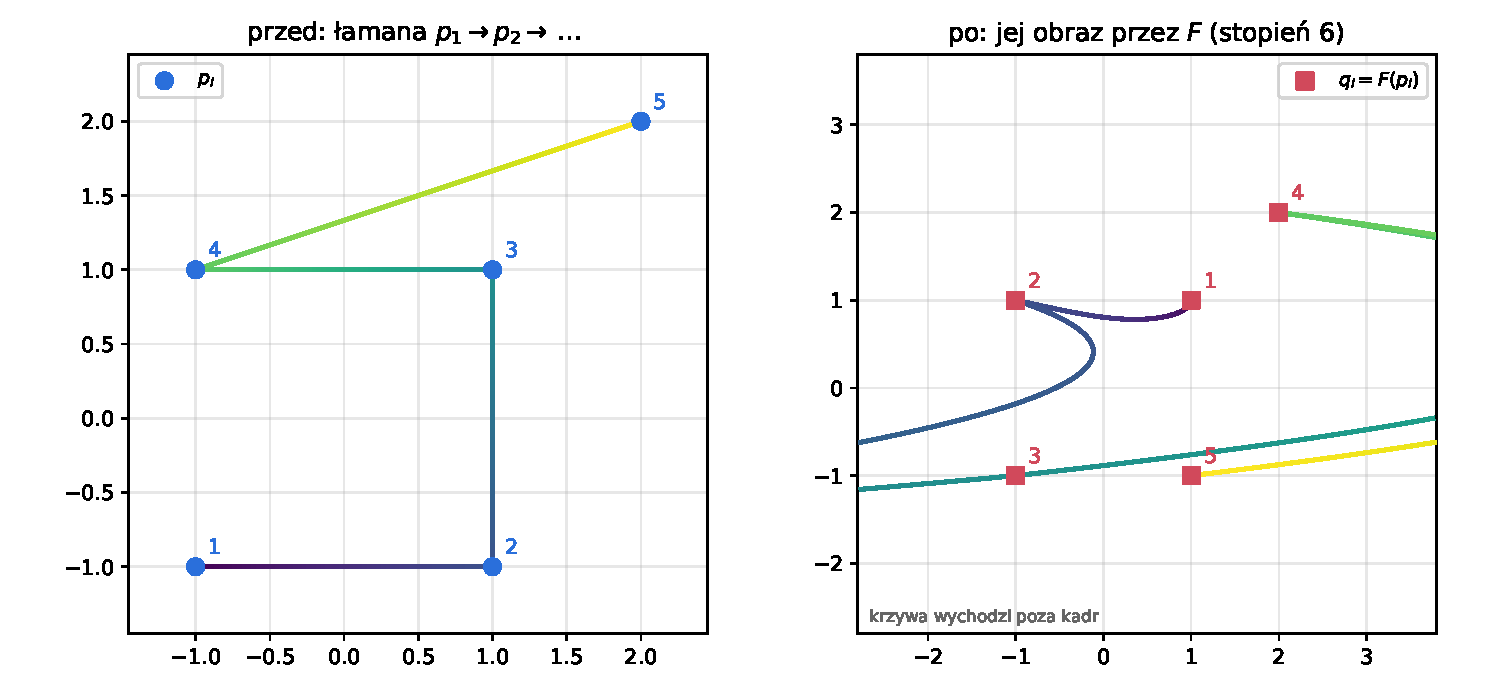
\includegraphics[width=\textwidth]{gen/najlepsze.pdf}\caption{Łamana $p_1\to\dots\to p_m$ (lewa) i jej obraz przez najlepsze znalezione $F$ (prawa); barwa wskazuje położenie wzdłuż łamanej.}\end{figure}}{}
\IfFileExists{gen/czynniki.pdf}{\begin{figure}[h!]\centering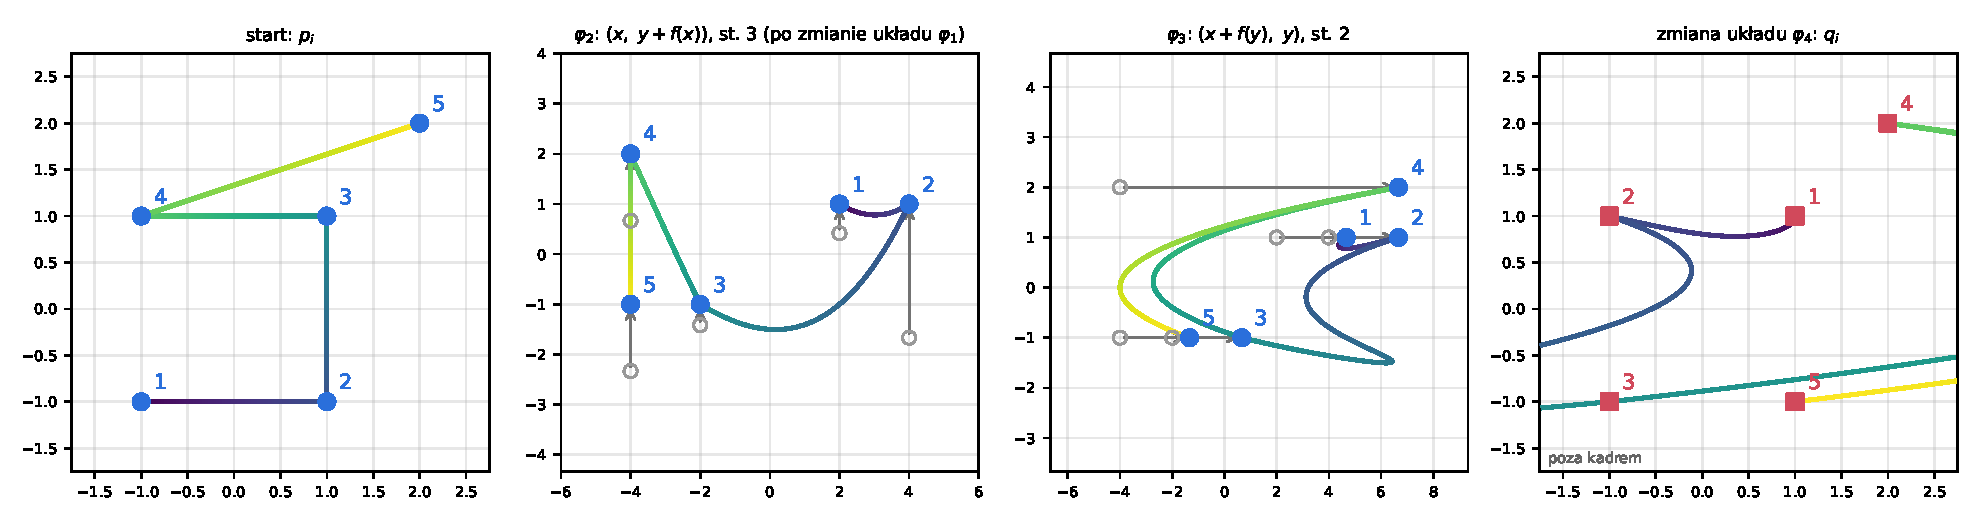
\includegraphics[width=\textwidth]{gen/czynniki.pdf}\caption{Działanie kolejnych czynników $\varphi_k$ najlepszego $F$ na punkty i łamaną. Czynnik trójkątny przesuwa punkty tylko pionowo albo tylko poziomo; każdy panel ma własny kadr.}\end{figure}}{}
\IfFileExists{gen/postep.pdf}{\begin{figure}[h!]\centering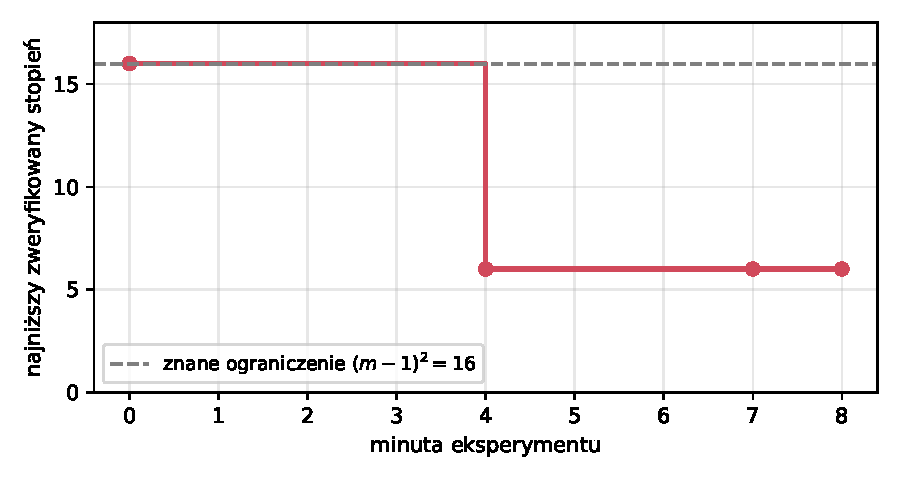
\includegraphics[width=0.7\textwidth]{gen/postep.pdf}\caption{Najniższy zweryfikowany stopień w kolejnych minutach eksperymentu.}\end{figure}}{}
